\subsubsection{探索词向量模型}
在上一步词向量模型训练完成后,我们来考察这个模型对于语义的理解。
首先来看看这个模型有没有区分不同语义实体的能力,探索结果如图\ref{fig:doesntsimilar}:
\begin{figure}[h]
\centering
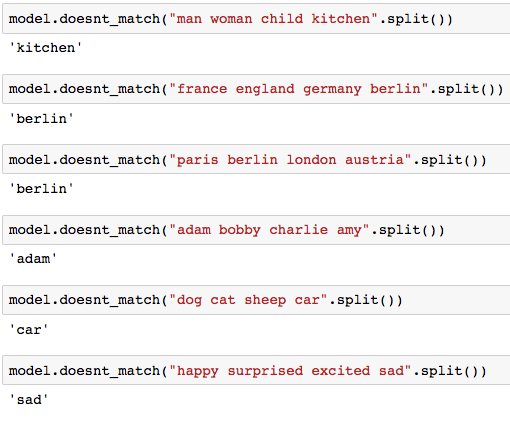
\includegraphics[width=0.9\linewidth]{doesnt_similar}
\caption[doesnt_similar]{探索词向量区分语义实体的能力}
\label{fig:doesntsimilar}
\end{figure}
从探索结果中可以看出,该模型对于语义实体的区分能力很不错。\\
之前也介绍说词向量模型可以通过向量空间距离关系来查找相似词,我们的探索结果如图\ref{fig:similar1}、图\ref{fig:similar2}、图\ref{fig:similar3}:
\begin{figure}[h]
\centering
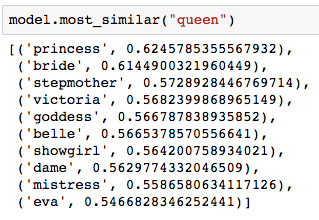
\includegraphics[width=0.8\linewidth]{similar1}
\caption[similar1]{探索词向量查找相似词的能力1}
\label{fig:similar1}
\end{figure}
\begin{figure}[h]
	\centering
	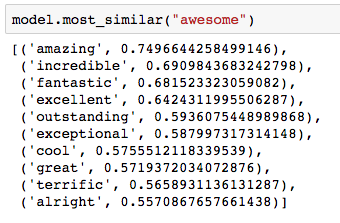
\includegraphics[width=0.8\linewidth]{similar2}
	\caption[similar2]{探索词向量查找相似词的能力2}
	\label{fig:similar2}
\end{figure}
\begin{figure}[h]
	\centering
	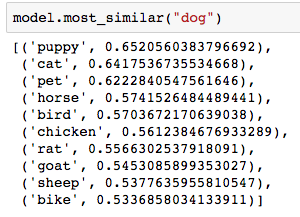
\includegraphics[width=0.8\linewidth]{similar3}
	\caption[similar3]{探索词向量查找相似词的能力3}
	\label{fig:similar3}
\end{figure}

从这几个探索的结果看来,词向量模型能够很好地查找出具有相似语义的词。
而这个相似不只是意思上的相似,还有语义实体在人类认知世界中概念分类上相似,如探索结果3,图\ref{fig:similar3}),相似词都是动物,更具体点是家畜类,而探索结果1,图\ref{fig:similar1},相似词都是女性角色。\\
从模型探索的结果来看,词向量模型弥补了词包模型对于语义理解的缺失,可以为特征提取工作提供更多有上下文含义的特征。\\